\subsection{Simulação para todo o ano de 2022}
\label{section: sim-2022}
Para simularmos o ano de 2022, os tempos médios entre chegadas para cada mês foram obtidos por meio de uma regressão exponencial, que ofereceu um modelo com $r^2$ de 0,99. A Figura \ref*{fig: regressao-expo-2022} mostra a tendência do tempo médio entre chegadas e a previsão de 12 valores, um para cada mês respectivo de 2022.\\
A estratégia de programação dos tempos foi idêntica à da Figura \ref*{fig: logica-2021}, apenas adaptando os dias úteis e os valores de média para 2022.\\
As simulações realizadas deram conta dos cenários de trabalho de 4 a 9 operadores, buscando avaliar as alternativas de contratação para a empresa ao longo de todo o ano de 2022.

\begin{figure}[H]
    \centering
    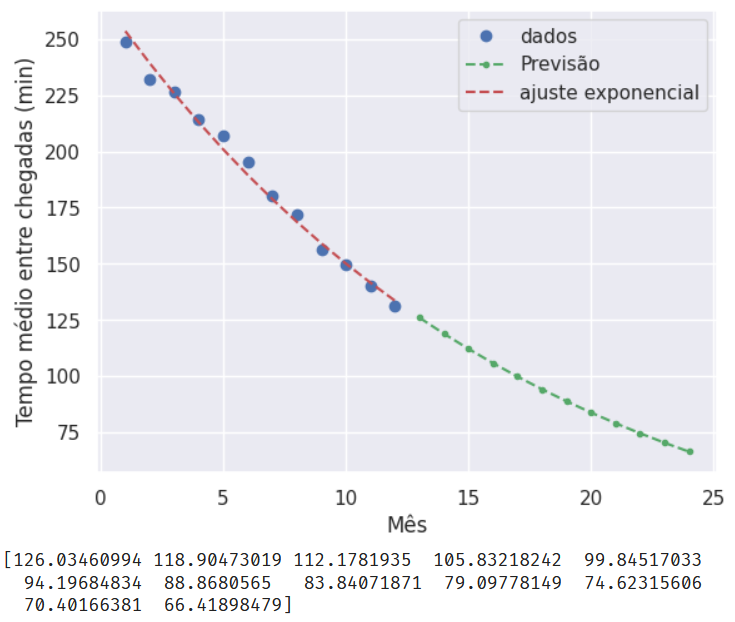
\includegraphics[scale=1]{simulacao/regressao-expo-2022.png}
    \caption{Regressão exponencial e previsão dos tempos entre chegadas para 2022}
    \label{fig: regressao-expo-2022}
\end{figure}
